\documentclass[12pt, a4paper, oneside, UTF8]{ctexart}
\usepackage{amsmath, amsthm, amssymb, bm, color, framed, graphicx, hyperref, mathrsfs}
\usepackage{geometry}
\geometry{left = 2.5 cm, right = 2.5 cm, top = 2.5 cm, bottom = 2.5 cm}

\title{\textbf{作业10}\\{\small (数值算法与案例分析)}}
\author{李维杰}
\date{\today}
\linespread{1.5}
\definecolor{shadecolor}{RGB}{241, 241, 255}
\newcounter{problemname}
\newenvironment{problem}{\begin{shaded}\stepcounter{problemname}\par\noindent\textbf{题目\arabic{problemname}. }}{\end{shaded}\par}
\newenvironment{solution}{\par\noindent\textbf{解答. }}{\par}
\newenvironment{note}{\par\noindent\textbf{注记. }}{\par}

\newcommand{\pll}{\kern 0.56em/\kern -0.8em /\kern 0.56em}

\begin{document}

\maketitle

\begin{problem}
    设$A$是一个Hermite阵.详细描述如何在应用隐式QR算法之前,把$A$酉相似变换为一个实三对角矩阵.
\end{problem}

\begin{solution}
    对于第$k$次循环,取Householder矩阵$H_k$,使得$A \leftarrow H_kA$后,有
    \begin{align*}
        \left\{
            \begin{array}{ll}
                A(k+1, k) \leftarrow {\left\lVert{A(k+1:n, k)}\right\rVert}_{2} \\
                A(k+2:n, k) \leftarrow 0
            \end{array}
        \right. ,
    \end{align*}
    则对称地,在$A \leftarrow AH_k$后,$A$阵上三角的对应部分同时会被消成$0$.
    上述过程循环$n-2$次,每次均做迭代$A \leftarrow H_kAH_k^*$,即得$$T = (H_{n-2}H_{n-3}...H_1)A(H_1...H_{n-3}H_{n-2})$$是一个三对角阵.
\end{solution}

\begin{problem}
    设$A,B$均为$n \times n$的实对称矩阵,其中$B$还是一个正定阵.证明:$AB$是可对角化的,并设计一种算法来计算$AB$的所有特征对.
\end{problem}

\begin{solution}
    对称正定阵$B$有Cholesky分解$B=LL^T$,于是有$$L^T AB (L^T)^{-1} = L^T A L.$$这表明$AB$相似于一个实对称阵,故$AB$是可对角化的.\par
    于是计算$AB$的所有特征对相当于计算实对称阵$L^T A L$的所有特征对,采用对称QR算法即可.
\end{solution}

\begin{problem}
    实现计算矩阵指数的scaling-and-squaring算法(结合截断Taylor级数).通过一些已知谱分解的可对角化矩阵来测试算法的准确性.
\end{problem}

\begin{solution}
    (图1代码见Problem3.m)
    \begin{figure}[htbp]
        \centering
        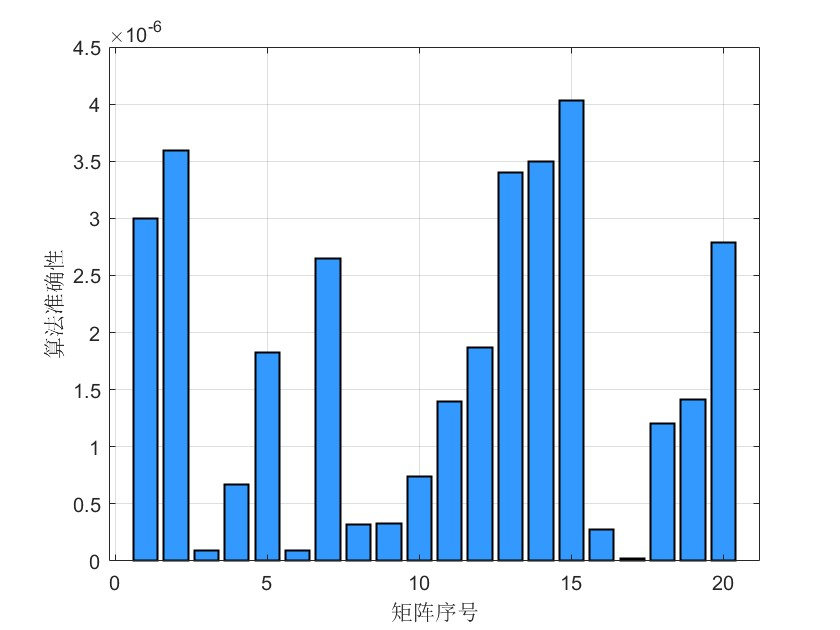
\includegraphics[scale=0.3]{Problem3.jpg}
        \caption{scaling-and-squaring算法的准确性${\left\lVert{(e^{\frac{A}{2^k}})^{2^k} - \text{expm}(A)}\right\rVert}_{\mathsf{F}}$}
    \end{figure}
\end{solution}

\begin{problem}
    设$A$和$E$是满足$AE=EA$的Hermite矩阵.尝试给出$${\left\lVert{\exp{(A+E)}-\exp{(A)}}\right\rVert}_{2}$$的上界.同时确保这个上界在${\left\lVert{E}\right\rVert}_{2} \rightarrow 0$时趋于$0$.
\end{problem}

\begin{solution}
    由于$A,E$均为Hermite矩阵,故$A,E$均可酉对角化.又$AE=EA$,故存在酉阵$U$,使得
    \begin{align*}
        D_A = UAU^* && D_E = UEU^* .
    \end{align*}
    设$D_A = \text{Diag}(a_1, a_2, ..., a_n)$, $D_E = \text{Diag}(e_1, e_2, ..., e_n)$, 并规定$a,e$均按从大到小的顺序顺次排列,则
    \begin{align*}
        {\left\lVert{\exp{(A+E)}-\exp{(A)}}\right\rVert}_{2} &= {\left\lVert{\exp{(D_A+D_E)}-\exp{(D_A)}}\right\rVert}_{2} \\
        &= {\left\lVert{\exp{(D_A)}(\exp{(D_E)}-I)}\right\rVert}_{2} \\
        &\leq {\left\lVert{\exp{(D_A)}}\right\rVert}_{2}{\left\lVert{\exp{(D_E)}-I}\right\rVert}_{2} \\
        &= \exp{(a_1)} (\exp{(e_1)} - 1) \\
        &= \exp{({\left\lVert{A}\right\rVert}_{2})}(\exp{({\left\lVert{E}\right\rVert}_{2})} - 1) .
    \end{align*}
\end{solution}

\begin{problem}
    复现附件论文中包含的实验.
\end{problem}
    
\begin{solution}
    (图2代码见Problem5\_1.m)
    \begin{figure}[htbp]
        \centering
        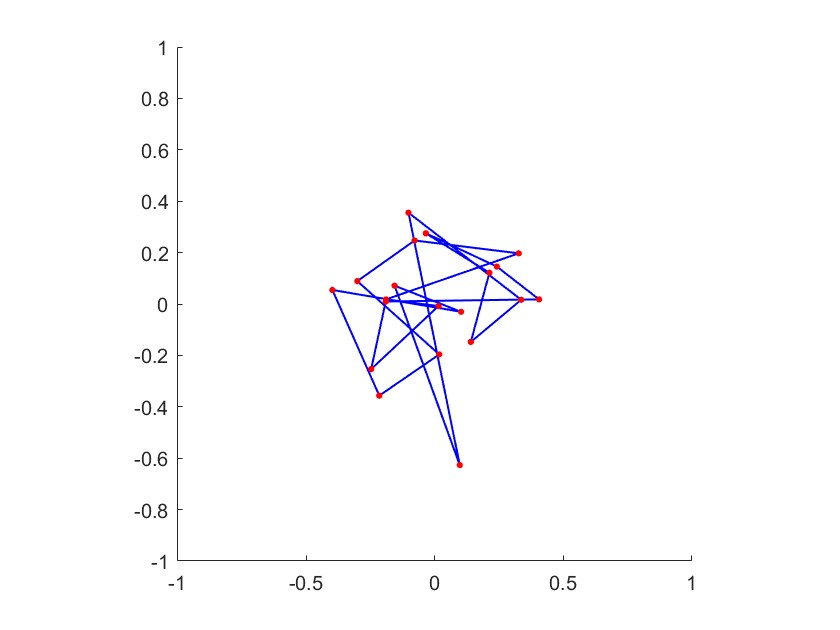
\includegraphics[width=0.3\textwidth]{Problem5.1.1.jpg}
        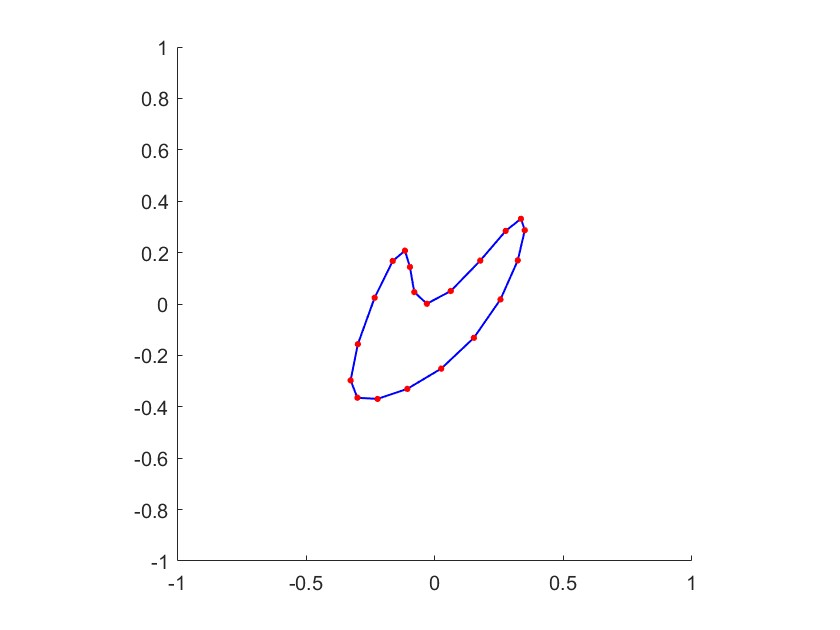
\includegraphics[width=0.3\textwidth]{Problem5.1.2.jpg}
        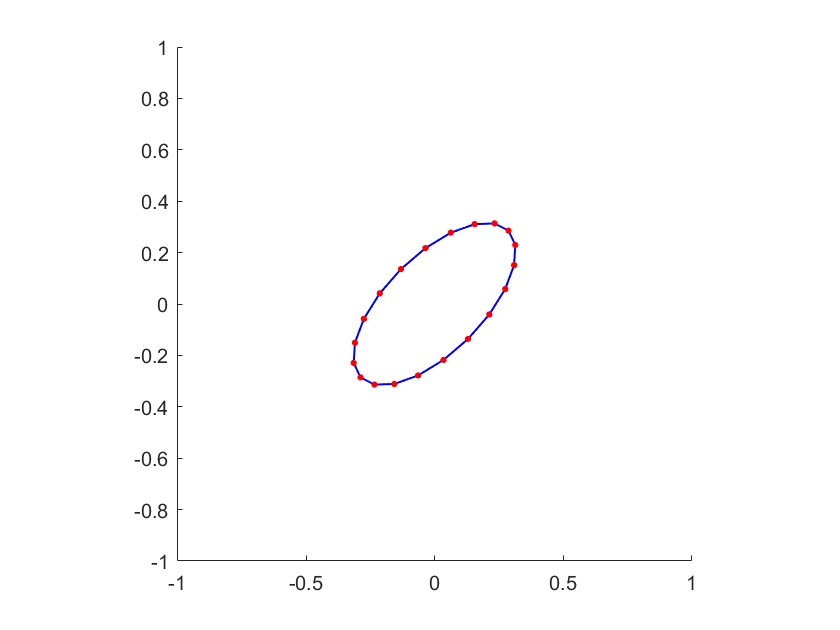
\includegraphics[width=0.3\textwidth]{Problem5.1.3.jpg}
        \caption{The progression from $P_{0}$ to $P_{18}$ to $P_{200}$ for an $n = 20$ example.}
    \end{figure}\\
    (图3代码见Problem5\_2.m,其中使用Problem5\_1.m的结果初始化$c$和$s$)
    \begin{figure}[htbp]
        \centering
        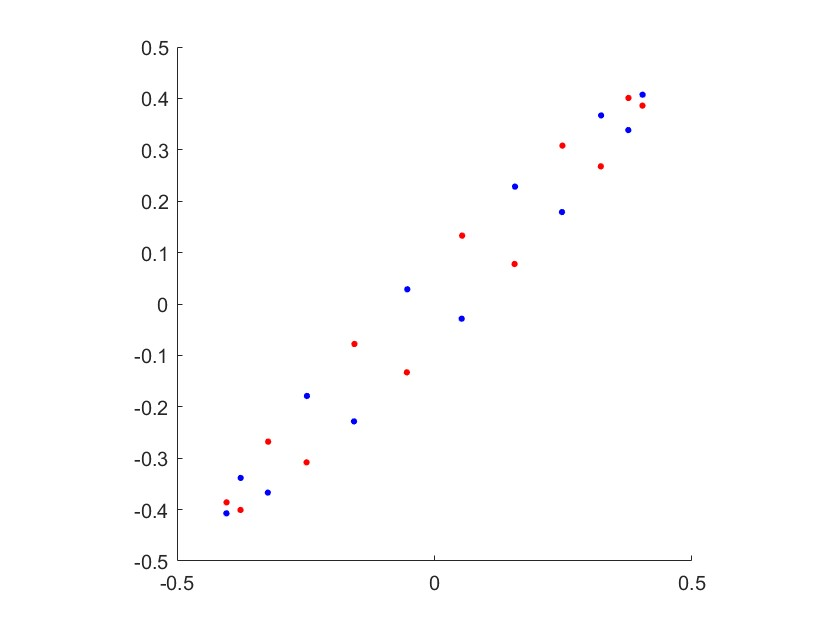
\includegraphics[scale=0.3]{Problem5.2.jpg}
        \caption{The vertices of $P_{even}$ (red) and $P_{odd}$ (blue) ($n = 12$)}
    \end{figure}
\end{solution}

\end{document}